\documentclass[12pt]{report}
\usepackage{lipsum} % For dummy text, you can remove this line
\usepackage{multicol}
\usepackage{hyperref}
\usepackage{shapepar}
\usepackage{amsmath}
\usepackage{amssymb}
\usepackage{xecolor}
\usepackage{upgreek}
\usepackage{pgfplots}
\usepgfplotslibrary{fillbetween}
\usepackage{xepersian}
\settextfont{XB Kayhan}

\setlength{\parindent}{10pt} 


\begin{document}
	

	\title{آنالیز ریاضی دکتر رضی}
	\author{پرهام طالبیان}
	\date{\today}
	\maketitle
	
	% Table of contents
	\tableofcontents
	
	
	% Chapter 1
	\chapter{انتگرال ریمان}
	\label{ch1}
	
	% Your content for Chapter 1 goes here
	\section{انتگرال پذیری ریمان }
	% Add your content here
	
	
	
	گیریم 
	$f:[a,b]\rightarrow\mathbb{R}$
	داده شده است به طور شهودی انتگرال 
	$f$
	روی 
	$[a,b]$
	،مساحت زیر نمودار آن است. یعنی
	
	
	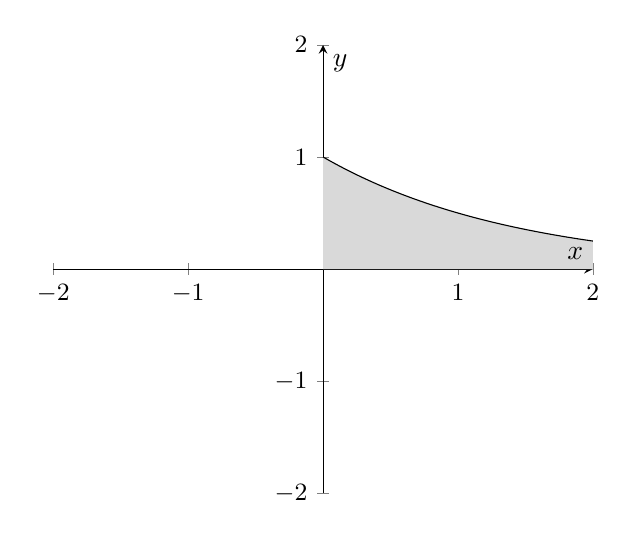
\begin{tikzpicture}
		\begin{axis}[
			xlabel={$x$},
			ylabel={$y$},
			xmin=-2, xmax=2,
			ymin=-2, ymax=2,
			axis lines=middle,
			ticklabel style={font=\small},
			]
			
			
			\addplot[name path=f, domain=0:2, smooth] {0.5^x};
			
			
			\addplot[name path=xaxis, domain=0:2, draw=none] {0};
		
			
			\addplot[gray!30] fill between[of=f and xaxis];
			
			
			
			
		\end{axis}
	\end{tikzpicture}
$\rightarrow S = \int_{a}^{b} f(x)\, \mathrm{dx}$



برای 
$f \geq 0$
داریم:

\[
	S = \int_{a}^{b} f(x)\, \mathrm{d}x
\]
که 
$S$
مساحت ناحیه هاشور خورده می‌باشد.


\textbf{تعریف:}
هر جفت افراز شامل دو مجموعه از نقاط،
$P,T \subseteq [a,b]$
است
$T = \{t_1, t_2, \dots, t_n\}$
عرض مستطیل و 
$P = \{x_0, x_1, x_2, \dots, x_n\}$
طول مستطیل که به صورت زیر با هم در ارتباط هستند:

\[
a = x_0 \leq t_1 \leq x_1 \leq t_2 \leq x_2 \leq \dots \leq t_n \leq x_n = b
\]
نقاط 
\, $x_0, x_1, x_2, \dots, x_n$\,
را متمایز می‌گیریم مجموع ریمان متناظر 
$f, P, T$
برابر است با
\[
R(f, P, T) = \sum_{i = 0}^n f(t_i) \Delta x_i
\]
که در آن 
$\Delta x_i = x_i - x_{i - 1}$
مجموع مساحت های مستطیل‌ هایی است که مساحت زیر خم $f$ را تقریب می‌زند.

\textbf{ظرافت افراز :P}
طول بزرگترین زیرفاصله 
$[x_{i - 1}, x_i]$
است هر افراز با ظرافت بزرگتر خشن و افراز با ظرافت کوچکتر ظرایف نامیده می‌شود.


\textbf{انتگرال پذیری ریمان:}
عدد حقیقی $l$ را انتگرال ریمان $f$ روی $[a, b]$ می‌نامیم هرگاه در شرط زیر صدق کند:
\[
\int_{a}^{b} f(x)\, \mathrm{d}x = l = \lim_{ \lVert \mathbf{P} \rVert \to 0} R(f, P, T)
\]
که معادل است با 
\[
\forall \varepsilon > 0 \,, \exists \delta > 0\, ; (\lVert \mathbf{P} \rVert < \delta \rightarrow |R - l| < \varepsilon)
\]
که به ازای هر افراز $P$ که ظرافت آن از $\delta$ کوچکتر است داشته باشیم\quad 
$|R(f, P, T)-l|< \varepsilon$

\textbf{قضیه:}
فرض کنید $f$ انتگرال پذیر ریمان باشد آنگاه $f$ کراندار است.

\textbf{اثبات:}
فرض کنید که $f$ کراندار نباشد در این صورت، فرض می‌کنیم 
$l = \int_{a}^{b} f(x) \mathrm{d}x$
چون $f$ انتگرال پذیر ریمان است
  
\[
\forall \varepsilon > 0 \,, \exists \delta > 0\, ; (\lVert \mathbf{P} \rVert < \delta \rightarrow |R - l| < \varepsilon)
\]
در این صورت با انتخاب
$\varepsilon = 1$





\begin{equation}\label{eq1}
	\forall \varepsilon > 0 \,, \exists \delta > 0\, ; (\lVert \mathbf{P} \rVert < \delta \rightarrow |R - l| < 1)
\end{equation}
فرض کنید جفت افراز 
$P, T$
به گونه ای باشد که 
$\lVert \mathbf{P} \rVert < \delta \, , |R - l| < 1$
اگر $f$ روی $[a, b]$ بی کران  باشد آنگاه حداقل یک زیر بازه 
$[x_{i - 1}, x_i]$
وجود دارد به طوریکه $f$ روی آن بی کران است. یک مجموعه جدید 
$T' = \{t'_1, t'_2, \dots, t'_n\} , t'_i = t_i$
 برای 
 $i \neq i_0$
 برمی‌گزینیم و
$t'_{i_0}$
را چنان برمی‌گزینیم که
\[
|f(t'_{i_0}) - f(t
_{i_0})|\,\Delta x > 2
\]
در این صورت قرار می‌دهیم 
$R'= R(f, P, T')$
که رابطه 
\,\eqref{eq1}\,
نتیجه می‌دهد
$|R' - l| < 1$
در این صورت خواهیم داشت 
$|R - R'| > 2$

\begin{equation}\label{eq2}
	|R - R'| = |f(t'_{i_0}) - f(t_0)|\Delta x_{i_0} > 2 
\end{equation}

\[
R = \sum_{i = 1}^n f(t_i) \Delta x_i \quad R' = \sum_{i = 1}^n f(t'_i) \Delta x'_i
\]
از طرفی چون 
$\lVert \mathbf{P} \rVert < \delta$	
است پس طبق فرض انتگرال پذیری ریمان برای تابع $f$ داریم 
\[
|R - l|<1 \,, |R' - l| < 1
\]
لذا خواهیم داشت:
\[
|R - R'| \leq |R-l|+|R'-l| < 2
\]
که در تناقض با رابطه
\eqref{eq2}
است.
\\~\\


$P = \{x_0 = a < x_1 < x_2 < \dots < x_n = b\}$ \quad
$T = \{t_1, t_2, \dots, t_n\}$


تابع
$f>0$
انتگرال پذیر ریمان روی 
 $[a, b]$
 است
$\iff$
\[\lim_{ \lVert \mathbf{P} \rVert \to 0} R(f, P, T)
\]

\[
\forall \varepsilon > 0 , \exists \delta>0 \qquad \forall P(\lVert \mathbf{P} \rVert < \delta \rightarrow |R-l|< \varepsilon)
\]

\textbf{تظریف:}
فرض کنید
$P$
 یک افراز از بازه دلخواه
$[a, b]$
باشد آنگاه افراز
 $P^*$
  تظریف $P$  می‌شود هرگاه
$P \subseteq P^*$
 





	\section{انتگرال پذیری داربو}
	% Add your content here
مجموع پایینی و بالایی یک تابع نسبت به افراز $P$ از
$[a, b]$
برابر است با 
\[
U(f, P) = \sum_{i = 1}^n M_i \Delta x_i \qquad , M_i = sup\{f(t) ; t \in [x_{i - 1}, x_i]\}
\]

\[
L(f, p) = \sum_{i = 1}^n m_i \Delta x_i \qquad , m_i = inf\{f(t) ; t \in [x_{i - 1}, x_i]\}
\]
\textbf{گزاره:}
فرض کنید $P'$ تظریف $P$ باشد تابع کراندار
$f:[a, b] \rightarrow \mathbb{R}$
$P , P'$
دو افراز از 
$[a, b]$
باشد به طوریکه
$P \subseteq P'$
در این صورت
\[
U(f, P') \leq L(f, P) \qquad L(f, P) \leq L(f, P') 
\]

\textbf{اثبات:}
فرض کنید
$ P' = P \cup \{w\}$

\[P = \{a = x_0 < x_1 < x_2 <\dots < x_n = b  \}
\]

چون 
$w \in [a, b]$
پس

\[
\exists i \, ; w\in [x_{i_0 - 1}, x_{i_0}] \quad ; x_{i_0 - 1} \,, x_{i_0} \in P
\]
\[
U(f, P) = \sum_{i = 1}^{n+1}  M_i \Delta x_i = \sum_{i = 1}^{i_{0} - 1} M_i \Delta x_i + (M_{i_0})' (w - x_{i_0 - 1}) + (M_{i_0})'' (x_{i_0} - w) + \sum_{i_0+1}^n M_i \Delta x_i
\]

جملات 
$U(f, P')$
دقیقا همان جملات
$U(f, P)$
است به غیر از جمله مربوط به زیر بازه 
$[x_{i - 1}, x_i]$
در
$U(f, p')$
جمله مربوط به زیر بازه
$[x_{i_0 - 1}, x_{i_0} ]$
به دو زیربازه 
$[x_{i_0 -1}, w] , [w, x_{i_0}]$
تقسیم می‌شود
\[
U(f, p) = \sum_{i = 1}^n M_i \Delta x_i = \sum_{i = 1}^{i_{0} - 1} M_i \Delta x_i + M_{i_0}(x_{i_{0}} - x_{i_0} - 1) + \sum_{i_0+1} M_i \Delta x_i
\] 

\textbf{تعریف:}
تابع کراندار
$f:[a, b] \rightarrow [-M, M]$
انتگرال پذیر است هرگاه
\[
 \forall \varepsilon >0\quad \exists P \in \overbrace{P[a, b]}^{\text{افراز های روی بازه a تا b}} ; U(f, P) - L(f, p) < \varepsilon
\]
\[
M_i = sup\{f(t) ; x_{i - 1} \leq t \leq x_i\} \qquad m_i = inf\{f(t) ; x_{i - 1} \leq t \leq x_i\}
\]
\[
U(f, P) = \sum_{i = 1}^n M_i\, \Delta x \qquad L(f, P) = \sum_{i = 1}^n m_i \, \Delta x
\]

\textbf{تعریف:}
انتگرال بالایی و پایینی تابع کراندار
$f:[a, b] \rightarrow [-M, M]$

\[
\bar{I}= \underset{\text{P}}{inf}\, U(f, p) \qquad \underbar{I} = \underset{\text{P}}{sup}\, L(f, p)
\]

\textbf{تعریف:}
تابع کراندار 
$f:[a, b] \rightarrow [-M, M]$
انتگال پذیر داربوست هرگاه
\[
\bar{I}=\underbar{I} = I
\]

\textbf{ تعریف :}
فرض کنید 
$P_1, P_2 \in P[a, b]$ 
در این صورت تظریف مشترک 
$P_1, P_2$
برابر است با
\[
P^* = P_1 \cup P_2
\]

\textbf{اصل تظریف:}	
تظریف هر افراز سبب افزایش مجموع پایین و کاهش مجموع بالایی می‌شود.

\textbf{نکته:}
طبق اصل تظریف داریم:
$\qquad \forall\,P_1, P_2 \in P[a, b]$

\[
L(f, P) \leq L(f, P^*)\leq U(f, P^*) \leq U(f, P)
\] 

\textbf{قضیه:}
انتگرال پذیری ریمان هم ارز (معادل) انتگرال پذیری داربوست.

\textbf{اثبات: }
فرض کنید تابع کراندار 
$f:[a, b] \rightarrow \mathbb{R}$
انتگرال پذیر داربوست ثابت می‌کنیم$ f$ ریمان انتگرال پذیر می‌باشد،کافیست ثابت کنیم

\[
\forall \,\varepsilon > 0 \quad \exists\,\delta > 0 \quad \forall\,P(\lVert \mathbf{P} \rVert < \delta \rightarrow |R - l| < \varepsilon)
\]
فرض کنید
$\varepsilon > 0$
، دلخواه چون
$f$
انتگرال داربوست به ازای 
$\varepsilon$


\begin{equation}\label{eq3}
	\exists P_1 \in P[a, b]\,;\, U(f, P_1) - L(f, P_1) < \frac{\varepsilon}{4}
\end{equation}
قرار می دهیم 
$\delta = \frac{\varepsilon}{8Mn_1}$
که
$n_1$
تعداد افراز 
$P_1$
است
فرض کنید 
$P \in P[a,b]$
به طوریکه
$\lVert \mathbf{P} \rVert < \varepsilon$.

فرض کنید 
$P^*$
تظریف مشترک 
$P , P_1$
است لذا داریم
$P^* = P_1 \cup P$
طبق اصل تظریف داریم
$L_1 \leq L^* \leq U^* \leq U_1$

\[
L_1 = L(f, P_1) \qquad L^* = L(f, P^*)
\]
\[
U^* = U(f, P^*) \qquad U_1= U(f, P)
\]
در این صورت طبق رابطه
\ref{eq3}
داریم
$U^* - L^* \leq \frac{\varepsilon}{4}$

فرض کنید
$P\{x_i\}, P^*\{x^*_j\}$
که 
$0 \leq j \leq n\, , \, o \leq i \leq n$

مجموع های
$U^* = \sum M^*_j \Delta x , U = \sum m_i \Delta x_i$ 
همانند اند بجز جمله هایی با شرایط
$x_{i - 1} < x^*_j < x_i$

حداکثر 
$n_1 - 2$
جمله با شرط بالا وجود خواهد داشت که اندازه هر کدام حداکثر
$M\delta$
است. در این صورت داریم
\begin{equation}\label{eq4}
	U- U^* < (n_1 - 2)2M\delta < \frac{\varepsilon}{4} \xrightarrow{\frac{\varepsilon}{8Mn_1}\text{جایگذاری}}
\end{equation} 
به روش مشابه می‌توان ثابت کرد
$l^* - l < \frac{\varepsilon}{4}$
پس
\[
U - L = (U - U^*) + (U^* - L^*) + (L^*  - L) < \frac{\varepsilon}{4} + \frac{\varepsilon}{4} + \frac{\varepsilon}{2}= \varepsilon
\]	

چون 
$R(f,P,T) , I$
هر دو به فاصله 
$[L , U]$
تعلق دارند لذا 
$|R - I| < \varepsilon$

برعکس فرض کنید 
$f$
روی
$[a,b]$
انتگرال پذیر ریمان است ثابت می‌کنیم
$f$
روی 
$[a, b]$
داریم انتگرال پذیر داربوست چون 
$f$
بر
$[a, b]$
انتگرال پذیر ریمان است لذا طبق قضایای کتاب 
$f$
بر 
$[a, b]$
کراندار است و فرص کنید 
$\varepsilon > 0$
دلخواه و از این پس ثابت باشد چون
$f$
انتگرال پذیری ریمان است لذا طبق تعریف به ازای
$\frac{\varepsilon}{4}$

\begin{equation}\label{eq5}
	\exists \, \delta > 0 \qquad \forall\,P(\lVert P \rVert < \delta \rightarrow |R - I| < \frac{\varepsilon}{4})
\end{equation}	
مجموعه های میانی:
$ T = \{t_i\} \,,  T'=\{t'_i\}$
وجود دارند بطوریکه هر
$f(t_i)$
چنان بر 
$m_i$
و هر
$f(t'_i)$
چنان بر 
$M_i$
نزدیک است بطوریکه
\[
R - L < \frac{\varepsilon}{4} \quad , \quad U - R' <\frac{\varepsilon}{4}
\]
\[
R = R(f, P, T) \quad , \quad R' = R(f, P, T')
\]
چون 
$\lVert P \rVert < \delta$
پس طبق رابطه
\ref{eq5}
\[
|R - I| <\frac{\varepsilon}{4} \quad , \quad |R' - I| < \frac{\varepsilon}{4}
\]
\[
(U - L) = (U - R') + (R' - I) + (I - R) + (R - L) < \varepsilon
\]
چون
$\bar{I} ,  I, \underbar{I}$
عدد های ثابت هستند متعلق به فاصله   
$[L , U]$
با طول کمتر از 
$\varepsilon > 0$
و چون 
$\varepsilon >0$
دلخواه بود لذا داریم:
$\qquad  \bar{I} =  I= \underbar{I}$
بنابراین 
$f$
انتگرال پذیر داربوست.

\textbf{قضیه:}
هر تابع پیوسته
$f:[a, b]\rightarrow \mathbb{R}$
ریمان انتگرال پذیر است.

فرض کنید
$\varepsilon > 0$
دلخواه و از این پس ثابت باشد چون 
$f$
پیوسته و
$[a, b]$
فشرده است لذا 
$f$
بر
$[a, b]$
پیوسته یکنواخت می‌شود لذا به ازای هر
$\varepsilon$
\begin{equation}\label{eq6}
	\exists\, \delta > 0 \quad \forall \,s, t \in[a, b]\,(|s- t| < \delta \rightarrow |f(t) - f(s)| < \frac{\varepsilon}{2(b - a)})
\end{equation}
فرض کنید$P$ افرازی با شرط 
$\lVert P \rVert < \delta$
باشد روی هر فاصله افراز
$[x_{i -1}, x_i]$
داریم:

\begin{equation}\label{eq7}
	M_i - m_i < \frac{\varepsilon}{b-a}
\end{equation}
\[
P = \{a = x_0 < x_1 < x_2 <\dots <x_n = b\} \qquad 1 \leq i \leq n
\]
\[
U - L = \sum_{i = 1}^n (M_i - m_i )\, \Delta x \overset{\eqref{eq6}}{<} \frac{\varepsilon}{b-a}
\sum_{i = 1}^n\, \Delta x = \varepsilon
\]
بنابر 
\eqref{eq6}
محک انتگرال پذیر داربوست تابع $f$ انتگرال پذیر ریمان است.



\textbf{مثال:}
ابتدا پیوستگی و سپس انتگرال پذیری توابع زیر را بررسی کنید.

\begin{equation*}
	X_Q(x) = 
	\begin{cases}
		1 & \text{if }\qquad x  \in \mathbb{Q} \\
		0 & \text{if }\qquad x \in  \mathbb{Q}^c\\
		
	\end{cases}
\end{equation*}

\begin{equation*}
	f(x) = 
	\begin{cases}
		\frac{1}{q} & \text{if }\qquad x = \frac{p}{q}  \in \mathbb{Q} \\
		0 & \text{if }\qquad x \in  \mathbb{Q}^c\\
		
	\end{cases}
\end{equation*}
\subsection{خواص انتگرال ریمان}
\textbf{قضیه:}
(خطی بودن انتگرال)

الف)مجموعه همه توابع ریمان انتگرال پذیر روی
$[a, b]$
یک فضای برداری است و 
\[
f\rightarrow \int_{a}^{b} f(x) \mathrm{d}x
\]

ب) تابع ثابت 
$h(x) = k$
انتگرال پذیر ریمان است و انتگرال آن برابر با
$k(b-a)$
می‌باشد.

\textbf{اثبات الف:}
چون مجموع های انتگرال بطور طبیعی خاصیت ترکیب خطی دارند لذا خواهیم داشت
\[
R(f + cg, P,T) = R(f,P,T) + cR(g, P, T)
\]
$f , g$
انتگرال پذیر ریمان،
$c$
 اسکالر دلخواه
\[
R(f, P, T) = \sum_{i = 1}^n f(t_i) \,\Delta x_i \quad , \quad R(g, P, T) = \sum_{i = 1}^n g(t_i) \Delta x_i
\]
\[
cR(g, P, T) = \sum_{i = 1}^n  c\, g(t_i) \, \Delta x_i
\]
\[
R(f, P, T) + cR(g, P, T) = \sum_{i = 1}^n (f(t_i) + cg(t_i)) \Delta x_i
\]

\begin{equation}\label{eq8}
	R(f+cg, P, T) = R(f, P, T) + cR(g, P, T)
\end{equation}
از طرفین رابطه
\eqref{eq8}
وقتی
$\lVert \mathbf{P} \rVert \to 0$
حد می‌‌گیریم در این صورت داریم
\[
\lim_{ \lVert \mathbf{P} \rVert \to 0} R(f + cg,P, T) = \lim_{ \lVert \mathbf{P} \rVert \to 0} R(f, P, T) + c\,\lim_{ \lVert \mathbf{P} \rVert \to 0} R(g, P, T)
\]
\[
\int_{a}^{b} (f+cg)(x) \mathrm{d}x = \int_{a}^{b} f(x) \mathrm{d}x + c\int_{a}^{b} g(x) \mathrm{d}x
\]
\textbf{اثبات ب:}
اگر 
$f(x) = k$
در این صورت
\[
\forall P \in P[a, b] \,,\,\forall T \quad R(f, P,T) = \sum_{i = 1}^n f(t_i) \Delta x_i= k\sum_{i = 1}^n \Delta x_i = k(b-a)
\]
در این صورت
\[
\int_{a}^{b} k \mathrm{d}x = \lim_{ \lVert \mathbf{P} \rVert \to 0} R(f, P,T) = \lim_{ \lVert \mathbf{P} \rVert \to 0} k(b-a) = k(b-a)
\]

\textbf{قضیه یکنوایی انتگرال:}
اگر 
$f, g$
در بازه
$[a, b]$
انتگرال پذیر ریمان باشد 
$f < g$
آنگاه
\[
\int_{a}^{b} f(x) \mathrm{d}x < \int_{a}^{b} g(x) \mathrm{d}x 
\]

\[
f \leq g \rightarrow R(f, P, T) \leq R(g, P, T) \overset{\lim_{ \lVert \mathbf{P} \rVert \to 0}}{\rightarrow}  \int_{a}^{b} f(x) \mathrm{d}x \leq \int_{a}^{b} g(x) \mathrm{d}x 
\]

\textbf{قضیه(خاصیت توابع انتگرال پذیر ریمان):}
اگر $f$ انتگرال پذیر ریمان روی 
$[a, b]$
باشد

$|f| \leq M$

\[
|\int_{a}^{b} f(x) \mathrm{d}x| \leq M (b-a)
\]
\textbf{اثبات:}
\[
|f(x)| \leq M \rightarrow -M \leq f(x) \leq M
\]
خاصیت یکنوای انتگرال
\[
\int_{a}^{b} -M \mathrm{d}x \leq \int_{a}^{b} f(x) \mathrm{d}x \leq \int_{a}^{b} M \mathrm{d}x \rightarrow -M(b-a)  \leq \int_{a}^{b} f(x) \mathrm{d}x \leq M(b-a)
\]
بنابراین داریم
\[
|\int_{a}^{b} f(x) \mathrm{d}x| \leq M (b-a)
\]

یک مجموعه 
$M \subseteq \mathbb{R} $
از اندازه صفر است هرگاه
\[
\forall \, \varepsilon \quad \exists \underbrace{\{(a_i, b_i)\}_{i=1}^{\infty}}_{ \text{پوشش شمارش پذیر}} s.t \, M \subseteq U_{i = 1}^{\infty} \, (a_i, b_i) \,,\, \sum_{i = 1}^{\infty} (b_i - a_i) \leq \varepsilon
\]
\textbf{مثال:}
هر زیرمجموعه  از مجموعه ای با اندازه صفر، از اندازه  صفر است.

\textbf{اثبات:}
\[
A \subseteq B \qquad measure(B) = 0 \rightarrow measure(A) = 0
\]
فرض کنید
$\varepsilon > 0$
دلخواه باشد چون 
$measure(B) = 0$
پس طبق تعریف
\[
\exists\{(a_i, b_i)\}_{i=1}^{\infty}  \,,\, B \subseteq U_{i = 1}^{\infty} \, (a_i, b_i) \,,\, \sum_{i = 1}^{\infty} (b_i - a_i) \leq \varepsilon
\]
چون 
$A \subseteq B$
پس 
$A \subseteq B \subseteq U_{i = 1}^{\infty} \, (a_i, b_i) \,,\, \sum_{i = 1}^{\infty} (b_i - a_i) \leq \varepsilon$
پس 
$measure(A) = 0$

\textbf{مثال:}
هر مجموعه متناهی از اندازه صفر است.

 فرض کنید
$Z = \{z_1, z_2, \dots, z_n\}$
مجموعه متناهی باشد فرض کنید 
$\varepsilon > 0$
دلخواه باشد
$(z_i - \frac{\varepsilon}{2n}, z_i + \frac{\varepsilon}{2n}) ; 1 \leq i\leq n$
بوضوح
$\{(z_i - \frac{\varepsilon}{2n}, z_i + \frac{\varepsilon}{2n})\}_{i = 1}^{n}$
پوششی برای
$z$
است و 
\[
\sum_{i = 1}^n (z_i + \frac{\varepsilon}{2n} - (z_i - \frac{\varepsilon}{2n}))  = \sum_{i = 1}^{n} \frac{\varepsilon}{n}  = \frac{\varepsilon}{n}  \times n = \varepsilon
\]
چون 
$\varepsilon > 0$
دلخواه است پس 
$z$
از اندازه صفر است.

\textbf{مثال:}
اجتماع شمارش پذیر از مجموعه های از اندازه صفر،از اندازه صفر است.

فرض کنید
$z_1, z_2, \dots$
دنباله ای از مجموعه هایی با اندازه صفر باشد و 
$z = U_{i = 1}^{\infty} z_i$

فرض کنید
$\varepsilon > 0$
دلخواه باشد آن گاه چون
$z_1$
از اندازه صفر است پس با مقدار شمارش پذیر از فاصله های
$\{a_{i1}, b_{i1}\}_{i =1}^{\infty}$
که 
$\sum_{i = 1}^{\infty}(b_{i1} - a_{i1})$
پوشانده می‌شود.

چون 
$z_2$
از اندازه صفر است پس با مقدار شمارش پذیر از فاصله های
$\{a_{i2}, b_{i2}\}_{i =1}^{\infty}$
بطوریکه
$\sum_{i = 1}^{\infty}(b_{i2} - a_{i2}) < \frac{\varepsilon}{4}$
پوشانده می‌شود.

چون
$z_j$
از اندازه صفر است پس با مقدار شمارش پذیر از فاصله های
$\{a_{ij}, b_{ij}\}_{i =1}^{\infty}$
بطوریکه
$\sum_{i = 1}^{\infty}(b_{ij} - a_{ij})<\frac{\varepsilon}{2^j}$
پوشانده می‌شود.

چون اجتماع شمارش پذیر از شماراها،شمارش پذیر است پس گردایه همه
$\{a_{ij}, b_{ij}\}_{i = 1}^{\infty}$
تشکیل پوششی باز برای
$z$
می‌دهد که طول ان برابراست با
\[
\sum_{j = 1}^{\infty}\sum_{i = 1}^{\infty} (b_{ij} - a_{ij}) \leq \sum_{j = 1}^{\infty} \frac{\varepsilon}{2^j} = \frac{\varepsilon}{2} + \frac{\varepsilon}{4}+\dots  = \varepsilon
\] 
جون 
$\varepsilon > 0$
دلخواه بود پس 
$z$
ازاندازه صفر است.

\textbf{مثال:}
مجموعه شمارش پذیر از اندازه صفر است.

\textbf{اثبات:}
چون مجموعه های شمارا، اجتماع آنها شمارش پذیر از تک عضوی ها هستند پس طبق مثال قبل از اندازه صفر است.

\textbf{مثال:}
مجموعه کانتور از اندازه صفر است.


$E_0 = [0, 1]$	

$E_1 = [0,\frac{1}{3}] \cup [\frac{2}{3}, 1]$

$\vdots$

$E_n$

$E = \cap_{n = 1}^{\infty} E_n$

فرض کنید 
$\varepsilon > 0$
دلخواه باشد در این صورت 
$\exists n \in \mathbb{N}\, ;\, (\frac{2}{3})^n < \varepsilon$
طبق خاصیت ارشمیدسی اعداد طبیعی عدد 
$n$
 در بالا حتما وجود مجموعه کانتور مشمول درون
 $2^n$
 فاصله بسته  مانند
 $I_1, I_2, \dots, I_{2^n}$
 است که هر یک به طول 
 $\frac{1}{2^n}$
 است.
 
هر فاصله بسته 
$I_i$
را به یک فاصله باز
$I_i \subseteq (a_i, b_i)$
توسعه می‌دهیم بطوریکه
$(b_i - a_i) < \frac{\varepsilon}{2^n}$
(چون 
$\frac{1}{3^n} < \frac{\varepsilon}{2^n}$
، طول 
$I_n$
ها برایر است با 
$\frac{1}{3^n}$
است پس می‌توان این انتخاب را انجام داد.) طول کل این
$2^n$
فاصله 
$(a_i, b_i)$
برابر با 
$\varepsilon$
است. چون 
$\varepsilon > 0$
دلخواه بود پس کانتور از اندازه صفراست.

\textbf{قضیه (لبگ ریمان):}
$f:[a, b] \rightarrow \mathbb{R}$
ریمان انتگرال پذیر است اگر و تنها اگر کراندار بوده و مجموعه نقاط ناپیوستگی اش از اندازه صفر باشد.

\textbf{نتایج:}

۱.هر تابع پیوسته انتگرال پذیر ریمان است.

۲.هر تابع یکنوا ریمان انتگرال پذیر است.

\textbf{اثبات:}
توابع یکنوا مجموعه نقاط ناپیوستگی اش حداکثر شمارا است  پس از اندازه صفر است بوضوح تابع یکنوای 
$f$ 
بر 
$[a, b]$
 کراندار است پس طبق لبگ ریمان انتگرال پذیری ریمان است.
 
 ۳.حاصلضرب دو تابع انتگرال پذیر ریمان،انتگرال پذیر ریمان است.
 
 \textbf{اثبات:}
 فرض کنید 
 $f, g$
 انتگرال پذیر باشد آنگاه
 $f, g$
 بر 
 $[a, b]$
 کراندارند پس 
 $f \times g$
  بر
 $[a, b]$
کراندارند.

مجموعه نقاط ناپیوستگی 
$D(f)=f$

مجموعه نقاط ناپیوستگی 
$D(g) = g$
 
$f, g$
بر
$[a, b]$
کراندار است  و مجموعه نقاط ناپیوستگی اش  از اندازه صفر است پس طبق لبگ ریمان 
$f\times g$
انتگرال پذیر ریمان است.
\[
D(f, g) \subseteq D(f) \cap D(g)
\]
\[
t \in D(f\times g) \rightarrow \lim_{x \to t} (f\times g)(x) \neq (f\times g)(t)
\]

۴.اگر
$f:[a, b]\rightarrow [c, d]$
انتگرال پذیر ریمان باشد
$\phi:[c, d]\rightarrow\mathbb{R}$
پیوسته باشد آنگاه 
$\phi$
بر
$[a, b]$
انتگرال پذیر ریمان است.
اگر
$\phi$
پیوسته باشد 
$\leftarrow D(\phi, f) \subseteq D(f)$
نقاط ناپیوستگی ،چون 
$\phi$
کراندار است و مجموعه نقاط ناپیوستگی 
$f, \phi$
از اندازه صفر است پس
$f, \phi$
انتگرال پذیر ریمان است




	\chapter{دنباله و سری های تابعی}
	\label{ch۲}
	\textbf{تعریف:}
	فرض کنید
	$\{f_n\}$
	دنباله ای از توابع باشند که بر مجموعه 
	$E$
	تعریف شده اند دنباله
	$\{(f_n(x))\}$
	از اعداد را به ازای هر 
	$x \in E$
	همگرا می‌گوییم در این صورت می‌توانیم تابع 
	$f$
	را
	\[
	f(x) = \lim_{n \to \infty} f_n(x) \qquad (x \in E)
	\]
	تعریف ‌کنیم.
	
	دراین صورت می‌گوییم
	$\{f_n\}$
	بر
	$E$
	همگراست و 
	$f$
	حد یا تابع حدی
	$\{f_n\}$
	می‌نامیم و به صورت خاص می‌گوییم
	$\{f_n\}$
	بر
	$E$
	به صورت نقطه به نقطه (نقطه وار) همگراست.
	
	\textbf{مثال:}
	\[
	f_n(x) = x^n \quad ; \quad 0\leq x \leq 1 \qquad \lim_{n \to \infty} f_n(x) = 0
	\]
	
	\begin{equation*}
	f_n(x) = x^n \quad ; \quad 0\leq x \leq 1 \qquad \lim_{n \to \infty} f_n(x)=
	\begin{cases}
		1 & \text{if }\qquad x = 0 \\
		0 & \text{if }\qquad 0\leq x \leq 1   \\
		
	\end{cases}
	= f(x)
	\end{equation*}

\[
S_{m , n} = \frac{m}{m+n} \qquad \lim_{n \to \infty} \lim_{m \to \infty} \frac{m}{m+n} = 1
\]

(پیوستگی منتقل نمیشه)(پوینت وایز پیوستگی را منتقل نمی‌کند)
\[
\lim_{m \to \infty} \frac{m}{m+n} = 0
\]
(مثال نقض را باید برای امتحان حفظ کنیم)
\[
f_n(x) = \frac{x^2}{(1+x^2)^n} \qquad \mathbb{R} \, \text{سری هندسی بازه}  
\]
(پیوستگی منتقل نمی‌شود)(پوینت وایز پیوستگی را منتقل نمی‌کند)

\begin{equation*}
\sum_{n = 1}^{\infty} f_n(x)=
\begin{cases}
	0 & \text{if }\qquad x = 0 \\
	1 + x^2 & \text{if }\qquad x \neq 0 \\
	
\end{cases}
\end{equation*}	

\textbf{مثال:}
به ازای 
$m \in \mathbb{N}$
قرار می‌دهیم:
\[
f_m(x) = \lim_{n \to \infty} (\cos\, m! \pi x)^{2n} 
\]
وقتی
$m!x$
صحیح باشد  آنگاه
$f_m(x) = 1$
به ازای مقادیر دیگر 
$x$
داریم: 
$f_m(x) = 0$
در این صورت 
\[
f(x) = \lim_{m \to \infty} f_m(x)
\]
اگر 
$x \in \mathbb{Q^c}$
به ازای هر 
$m$
،
$f_m(x) = 0$
لذا
$f(x) = 0$

به ازای 
$x \in \mathbb{Q}$
مثلا
$x = \frac{p}{q}$
که در آن 
$ p , q \in \mathbb{Z} \quad$

اگر 
$m \geq q$
آنگاه 
$m!x$
صحیح است پس 
$f_m(x) = 1$
لذا
$f(x) = 1$

\begin{equation*}
	 \lim_{m \to \infty}\lim_{n \to \infty} (\cos\, m! \pi x)^{2n} =
	\begin{cases}
		0 & \text{if }\qquad x \in \mathbb{Q^c} \\
		1 & \text{if }\qquad  x \in \mathbb{Q}\\
		
	\end{cases}
\end{equation*}

\[
m = 2 \quad x = \frac{1}{7} \qquad f_n(x) = \lim_{n \to \infty} \cos 2 \pi )
\]

\textbf{مثال:}
فرض کنید
$f_n(x) = \frac{\sin(nx)}{\sqrt n}$

\[
\lim_{n \to \infty} f_n(x) = f(x) = 0 \qquad f'(x) = 0
\]
\[
f'(x) = \frac{\mathrm{d}(f_n(x))}{\mathrm{d}x} = \frac{1}{\sqrt n} \times n \cos (nx) = \sqrt n \cos(nx)
\]
که حد آن در بی نهایت وجود ندارد پس
\[
(\lim_{n \to \infty} f_n(x))' \neq \lim_{n \to \infty} (f_n(x))'
\] 
\textbf{مثال:}
\[
f_n(x) = n^2 (1 - x^2)^n \, ,\, 0 \leq x \leq 1
\]

\begin{equation*}
	f(x) =
	\begin{cases}
		0 & \text{if }\qquad x = 0 \\
		0 & \text{if }\qquad  0 \leq x \leq 1\\
		
	\end{cases}
\end{equation*}
\[
\lim_{n \to \infty} f_n(x) = f(x) = 0
\]
\[
\int_{0}^{1} f(x) \,\mathrm{d}x = \int_{0}^{1} 0\, \mathrm{d}x = 0
\]
\[
n \in \mathbb{N} \qquad \int_{0}^{1} f_n(x)\,\mathrm{d}x = \int_{0}^{1} n^2 (1 - x^2)^n \,\mathrm{d}x = n^2 \int_{0}^{1} x (\frac{1 - x^2}{6})^n \,\mathrm{d}x = \frac{n^2}{2n + 2}
\]
\textbf{ تعریف همگرایی یکنواخت:}
دنباله تابعی 
$f_n(x)$
به صورت یکنواخت به
$f(x)$
همگراست هرگاه
\[
 U. \rightarrow \forall \varepsilon > 0 \, , \, \exists N \,\,\, \forall n \,,\, \forall x   \in D_f (n  \geq N \rightarrow |f_n(x) - f(x)| < \varepsilon)
\]
\[
f_n(x)  \overset{u.}{\rightarrow} f(x) \qquad f_n(x)  \overset{P.w.}{\rightarrow} f(x)
\]

\[
 P.W. \rightarrow \forall \varepsilon > 0 \, ,\, \forall x \in D_f \,,\, \exists N_x \,,\, \forall n   \in D_f (n  \geq N_x \rightarrow |f_n(x) - f(x)| < \varepsilon)
\]
\[
x^n ; 0 < x < 1
\]


\section{محک ها برای همگرایی یکنواخت}


\textbf{محک اول (کوشی):}
 دنباله ای از توابع مانند 
$\{f_n\}$
تعریف شده بر
$E$
به طور یکنواخت بر 
$E$
 همگراست اگر و تنها اگر به ازای هر
 $\varepsilon > 0$
 عدد صحیحی مانند 
 $N$
  وجود داشته باشد به طوریکه
  \[
  m , n \geq N \quad , \quad x \in E \qquad |f_n(x) - f_m(x)| \leq \varepsilon
  \]
  
  \textbf{اثبات:}
  فرض کنید 
  $f_n(x)  \overset{u.}{\rightarrow} f(x)$
  
  فرض کنید 
  $\varepsilon > 0$
  دلخواه و ثابت باشد طبق تعریف همگرایی یکنواخت
  \[
   \exists N \,\,\, \forall n \, \forall x\, (n  \geq N \rightarrow |f_n(x) - f(x)| < \frac{\varepsilon}{2}
  \]
  
  فرض کنید 
  $m \geq n $
  در این صورت داریم:
  \[
  |f_n(x) - f_m(x)| \leq |f_n(x) - f(x)| + |f_m(x) - f(x)| < \frac{\varepsilon}{2} + \frac{\varepsilon}{2} = \varepsilon
  \] 
  
  \textbf{اثبات عکس:}
  فرض کنید شرط کوشی برقرار باشد آنگاه دنباله
  $\{f_n(x)\}$
  به  ازای هر 
  $x$
   یک دنباله کوشی است پس به 
   $f(x)$
   همگرا می‌شود باید ثابت کنیم
   $f_n(x)  \overset{u.}{\rightarrow} f(x)$
   
   فرض کنید 
   $\varepsilon > 0$
   دلخواه و از این پس ثابت باشد طبق فرض کوشی داریم
   \[
   \exists N \, \forall n, m \, \forall x(n , m  \geq N \rightarrow |f_n(x) - f_m(x)| \leq \varepsilon)
   \]
   در رابطه بالا 
   $n$
   را ثابت گرفته و 
   $m$
   را به بی نهایت میل دهید در این صورت 
   $f_m(x) \rightarrow f(x)$
   و پس داریم:
   \[
   \forall x \,, \, \forall n \, (n \geq N \rightarrow |f_n(x) - f_m(x)| < \varepsilon)
   \]
   

مثالی که در فضای دیگری کوشی است اما همگرا نیست:
$\frac{[nx]}{n} \rightarrow x \in \mathbb{Q^c} \qquad \{\frac{[nx]}{n}\} \subseteq \mathbb{Q}$	

\textbf{محک دوم:}
قضیه فرض کنید
$\lim_{n \to \infty} f_n(x) = f(x) \quad (x \in E)$
قرار می‌دهیم:
\[
M_n = sup |f_n(x) - f_m(x)| \qquad x \in E
\]
در این صورت 
$f_n  \overset{u.}{\rightarrow} f$
اگر و تنها اگر
$M_n \rightarrow 0$

مثال:

\[
f_n(x) = \frac{1}{nx + 1} \qquad M_n = \underset{x \in D_f}{sup}|f_n(x) - f(x)| \, , \, f(x) = 0
\]
\[
n = 1 , \, M_1 = \underset{0 < x <1}{sup}|f_1(x)|=  \underset{0 < x <1}{sup}|\frac{1}{x + 1}| = 1
\]
\[
n = 2 , \, M_2 = \underset{0 < x <1}{sup}|f_2(x)|= \underset{0 < x <1}{sup}|\frac{1}{2x + 1}| = 1
\]
\[
n = 3 , \, M_3 = \underset{0 < x <1}{sup}|f_3(x)|= \underset{0 < x <1}{sup}|\frac{1}{3x + 1}| = 1
\]

\textbf{(آزمون وایرشتراس)قضیه:}
فرض کنید
$\{f_n\}$
دنباله ای از توابع باشد که بر 
$E$
تعریف شده است
\begin{equation}\label{eq9}
|f_n(x)| \leq M_n
\end{equation}

در این صورت اگر 
$\sum_{n = 1}^{\infty} M_n$
 همگرا شود آنگاه
 $\sum_{n = 1}^{\infty} f_n(x)$
 به طور یکنواخت همگرا می‌شود.
 
\textbf{اثبات:}
از آنجایی که 
$\sum_{n = 1}^{\infty} M_n$
همگراست داریم.(محک کوشی)
\[
\forall \varepsilon > 0 \quad \exists N \quad, \forall m, n \,\,(m , n \geq N \rightarrow \underbrace{\sum_{i= n}^{m} M_i}_{|s_m - s_n|} < \varepsilon)
\]
در این صورت از نامساوی 
$\eqref{eq9}$
داریم:
\[
\sum_{i= n}^{m} |f_i(x)| \leq \sum_{i= n}^{m} M_i}< \varepsilon
\]
پس طبق محک کوشی  
 $\sum_{n = 1}^{\infty} f_n(x)$
 به صورت یگنواخت همگرا می شود.
 
 
\textbf{قضیه:}
فرض کنید در یک فضای متری
$f_n \rightarrow f$
به طور یکنواخت بر مجموعه 
$E$
همگرا می‌شود.
$x$
را یک نقطه حدی 
$E$
در نظر می‌گیریم و فرض می‌کنیم
\begin{equation}\label{eq10}
	\lim_{t \to x} f_n(t) = A_n \qquad (n \in \mathbb{N})
\end{equation}

در این صورت 
$\{A_n\}$
همگراست و 
\begin{equation}\label{eq11}
	\lim_{t \to x} f(t) = \lim_{n \to \infty} A_n
\end{equation}
\
به عبارت دیگر :
\[
\lim_{t \to x} \lim_{n \to \infty} f_n(t) = \lim_{n \to \infty} \lim_{t \to x} f_n(t)
\]

\textbf{اثبات:}
فرض کنید
$\varepsilon$
 دلخواه و از این پس ثابت باشد چون 
 $f_n(x)  \overset{u.}{\rightarrow} f(x)$
 طبق محک کوشی
 
 \begin{equation}\label{eq12}
 	\exists N \quad \forall m ,n \, , \, \forall t \in E (m, n > N \rightarrow |(f_n(t) - f_m(t)|< \varepsilon) 
 \end{equation}

در این صورت با فرض 
$t \to x$
در رابطه 
$\eqref{eq12}$
داریم:
\[
\forall m , n\,(m, n > N \rightarrow |A_n - A_m| < \varepsilon)
\]
پس 
$\{A_n\}$
دنباله کوشی و فضای ما کامل است 
$(\mathbb{R} , \mathbb{R}^2)$
\begin{equation}\label{eq13}
	A_n \rightarrow A
\end{equation}

\begin{equation}\label{eq14}
	|f(t) - A| < |f(t) - f_n(t)| + |f_n(t) - A_n| + |A_n - A|
\end{equation}

فرض کنید 
$\varepsilon > 0$
 دلخواه و از این پس ثابت باشد چون
$f_n  \overset{u.}{\rightarrow} f$

\[
\frac{\varepsilon}{3} \exists N_1 \quad \forall n \quad \forall t \, (n > N_1 \rightarrow |f_n(t) - f(t)|<\frac{\varepsilon}{3})
\]
چون 
$A_n \rightarrow A$
\[
\frac{\varepsilon}{3} \exists N_2 \quad \forall n  \, (n > N_2 \rightarrow |A_n - A|<\frac{\varepsilon}{3})
\]
طبق رابطه 
$\eqref{eq10}$

\[
\frac{\varepsilon}{3} \exists V_x \quad \forall t \in V_x \cap E\, (|f_n(t) - A_n| <\frac{\varepsilon}{3} )
\]
لذا با قرار دادن نامساوی های فوق در رابطه 
$\eqref{eq14}$
داریم و با فرض

$ n > max\{N_1 , N_2\} \qquad t \in V_x \cap E$

داریم:
\[
|f(t) - A| < \frac{\varepsilon}{3} + \frac{\varepsilon}{3} + \frac{\varepsilon}{3} = \varepsilon
\]
چون 
$\varepsilon$
دلخواه است لذا حکم برقرار است.

\textbf{قضیه:}
فرض کنید که
$k$
فشرده باشد
$\{f_n\}$
دنباله ای از توابع پیوسته بر 
$k$
باشد 
$\{f_n\}$
به صورت نقطه وار به تابع پیوسته 
$f(x)$
همگرا شود به ازای هر
\[
 f_n(x) \geq f_{n + 1}(x) \quad x \in k \quad, \quad n \in \mathbb{N}
\]
آنگاه 
$f_n(x)  \overset{u.}{\rightarrow} f(x)$

\textbf{اثبات:}
قرار می‌دهیم:

$g_n = f_n - f$
پس 
$g_n$
پیوسته است و 
$g_n \to 0$
به صورت نقطه وار 
\[
g_n(x) \geq g_{n+1}(X)\,\, ;\,\, \forall x \in k \, ,\, n \in \mathbb{N}
\]
کافیست ثابت کنیم
$g_n(x)  \overset{u.}{\rightarrow} 0$.

فرض کنید
$\varepsilon > 0$
دلخواه و از این پس ثابت باشد
\begin{center}
$k_1 = \{x \in k \, , \, g_1(x) \geq \varepsilon\}$

$k_2 = \{x \in k \, , \, g_2(x) \geq \varepsilon\}$

$\vdots$ 

$k_n = \{x \in k \, , \, g_n(x) \geq \varepsilon\}$

$\vdots$ 
\end{center}
لذا
$k_1 , k_2 , \dots , k_n , \dots$
زیرمجموعه بسته از مجموعه فشرده 
$k$
هستند و لذا فشرده اند از آنجایی که 
$\{g_n(x)\}$
نزولی است داریم:
\[
k_1 \supseteq k_2 \supseteq k_3 \supseteq \dots 
\]
$x\in k$
را ثابت می‌گیریم چون
$g_n  \overset{p.w}{\to} 0$

لذا 
$\forall n \,(n > N \rightarrow x \notin k _n)$
پس
$ \varnothing = \cap_{n = 1}^{\infty} k_n$
لذا حداقل یکی از 
$k_N$
ها تهی خواهد شد لذا داریم به ازای 
\[
\forall x\in k \,, \, \forall n \,(n > N \rightarrow |g_n(x)| < \varepsilon)
\]
و لذا 
$g_n  \overset{u.}{\to} 0$

\textbf{تعریف:}
فرض کنید 
$\uptau(X)$
مجموعه توابع مختلط مقدار پیوسته و کراندار بر
$X$
باشد در این صورت
\[
\forall f \in \mathcal{C} \,;\, \lVert f \rVert = \underset{x \in y}{sup}|f(x)|
\]
$\uptau(X)$
با متر زیر فضای متریک است
$d(f, g) = \lVert f - g \rVert$

\textbf{قضیه:}
$\uptau$
با متر فوق یک فضای متریک کامل است.


\textbf{اثبات:}
فرض کنید 
$\{f_n\}$
یک دنباله کوشی  در 
$\uptau(X)$
باشد پس
\[
\forall \varepsilon > 0 \quad \exists N \,\, \forall n , m \, (m ,n > N \rightarrow \lVert f_n - f_m \rVert  < \varepsilon)
\]
در این صورت طبق محک کوشی 
$n_n  \overset{u.}{\rightarrow} f(x)$
در این صورت از قضایای قبلی چون
$f_n$
ها به صورت یکنواخت به 
$f(x)$
همگرا هستند و 
$f_n$
ها همگی پیوسته هستند لذا 
$f(x)$
پیوسته ، بوضوح مختلط مقدار می‌باشد
\[
\varepsilon = 1 \quad \exists N \quad \forall n , \forall x (n > N \rightarrow |f_n(x) - f(x) < 1) 
\]
\[
\rightarrow |f(x)| - |f_n(x)| \leq |f_n(x) - f(x)| < 1 \rightarrow |f(x)| \leq \underbrace{|f_n(x)|}_{\text{کراندار}} + 1
\]
لذا 
$f(x)$
کراندار است پس
$f(x) \in \uptau(x)$
پس 
$\uptau(x)$
کامل است.
$$

 \textbf{(پایان مباحث میانترم)}

 \section{همپیوستگی}
 
 \quad\textbf{تعریف:}
 خانواده
 $\mathcal{F}$
 از توابع مختلط
$f$
 تعریف شده بر مجموعه
$E$
 را در فضای متریک
$\mathcal{X}$
 در نظر بگیرید. در این صورت گوییم 
$\mathcal{F}$
  بر
$E$
همپیوسته است اگر


\textbf{نکته:}
 با توجه به تعریف هر یک از توابع
 $f\in\mathcal{F}$
 که در آن 
 $\mathcal{F}$
 خانواده ای از توابع مختلط مقدار باشد، به طور یکنواخت پیوسته هستند.
\\\par
 
 \textbf{تعریف:}
 فرض کنید 
 $\{f_n\}$
 مجموعه ای از توابع باشد که بر مجموعه 
 $E$
 تعریف شده است. گوییم
 $\{f_n\}$
 بر
 $E$
 به صورت 
 {\xecolor{red}  نقطه‌وار کراندار}
  است هرگاه دنباله 
  $\{f_n\}$
 به ازای هر
 $x\in E$
 کراندار باشد، یعنی تابعی با مقادیر متناهی چون 
 $\varPhi$
که بر 
$E$
تعریف شده، وجود داشته باشد به طوری که 
 \[
 |f_n(x)| < \varPhi (x) \quad (x\in E, n\in \mathbb{N})
 \]
 به علاوه گوییم
   $\{f_n\}$
   بر
   $E$
   به طور
{\xecolor{red}  یکنواخت کراندار}
    است هرگاه 
  \[
 \exists M>0 ;\;|f_n(x)| < M \quad (x\in E, n\in \mathbb{N}).
 \]
 
 \par
 
 \textbf{قضیه:}
 هرگاه
 $\{f_n\}$
 یک دنباله نقطه‌وار کراندار از توابع مختلط بر مجموعه شمارش پذیر 
 $E$ 
 باشد آنگاه 
 $\{f_n\}$
  زیر دنباله ای مانند 
 $\{f_{n_{k}}(x)\}$
 دارد که به ازای هر 
 $x$
 همگرای نقطه وار است.
 
  \textbf{اثبات:}
  فرض کنید
  $\{x_j\}$
  که 
  $i\in \mathbb{N}$
   به طوری که 
 $x_j$
  نقاط 
  $E$
  هستند که به صورت یک دنباله آراسته شده اند.
  
  ($\{x_j\}$
    یک شمارش یا enumeration 
    از اعضای مجموعه 
    $E$ 
    هستند.)
    
    
    
 
...
\par

بنابر این وقتی در آرایه فوق از یک سطر به سطر بعد می رویم. ممکن است توابع به چپ منتقل شود ولی هرکز به راست منتقل نمی شود.
در اینصورت اگر در امتداد قطر آرایه به پایین حرکت کنیم به دنباله 
$$
...
$$

می رسیم. بنابر ویژگی (۳)، دنباله S یک زیر دنباله از 
$S_n$
است و بنابر (۲) به ازای هر
$x \in E$
همگراست. پس 
$\{f_n(x)\}$
زیر دنباله ای مانند
$S$
پیدا کرد که به صورت نقطه وار همگراست.


$\\$
\par

\textbf{قضیه:}
هرگاه
 $k$
فشرده باشد و
$f_n\in\uptau(K)$
و
$\{f_n\}$
بر
$K$
به طور یکنواخت همگرا باشد، آنگاه
$\{f_n\}$
همپیوسته هستند.
\par

\textbf{اثبات:}
فرض کنید 
$\varepsilon>0$
دلخواه و از این پس ثابت باشد. چون 
$\{f_n\}$
به طور یکنواخت همگرا هستند پس چون 
$f_n(x)\xrightarrow[]{u}f(x)$
طبق محک کوشی داریم
   \[
 \exists N\quad\forall n,m \quad\forall x\in K (n,m \geq N \Rightarrow |f_n(x) - f_m(x)| < \varepsilon)
\]
در اینصورت چون 
$f_n$
ها پیوسته هستند و دامنه آنها فشرده است، پس طبق قضایای آنالیز داریم
$f_n$
ها بر 
$K$ 
پیوسته یکنواخت هستند.

پس به ازای 
$\varepsilon>0$
دلخواه، وجود دارد
$\delta>0$
به طوری که اگر
\[
1\leq i\leq\mathbb{N}\quad
(d(x, y)<\delta \Rightarrow |f_i(x)-f_i(y)|<\varepsilon)
\]
در این صورت اگر


\[
\vdots
\]

\textbf{قضیه(استون وایرشتراس):}
هرگاه 
$f$
تابع مختلط پیوسته ای بر
$[a,b]$
 باشد دنباله‌ای از چند جمله ای ها مانند 
 $\{P_n\}$
 وجود دارد بطوریکه 
 $\lim_{n \to \infty} P_n(x) = f(x)$
 به طور یکنواخت بر 
 $[a, b]$
 اگر 
 $f$
 تابعی حقیقی بر
 $[a, b]$
 باشد می‌توان 
 $\{P_n\}$
 را حقیقی بدست آورد.
 
\textbf{نتیجه:}
له ازای هر بازه 
$[-a , a]$
دنباله ای از چند جمله ای های حقیقی مانند
$\{P_n\}$
 وجود دارد بطوریکه
\[
P_n(0) = 0 ; \forall n \in \mathbb{N} \qquad , \qquad \lim_{n \to \infty} P_n(x) = |x|
\]
بر 
$[-a, a]$
بطور یکنواخت

\textbf{اثبات:}
طبق قضیه استون-وایرشتراس چند جمله حقیقی 
$\{P^*_n\}$
وجود دارد که
$\lim_{n \to \infty} P^*_n(x) = |x| $
\[
P_n(x) = P_n^*(x) - P_n^*(0)
\]
\[
p_n(0) = P_n^*(0) - P_n^*(0) = 0
\]
در این صورت خواهیم داشت
\[
\lim_{n to \infty} P_n(x) = |x| \quad , \quad P_n(0) = 0 \quad ; \quad \forall n \in \mathbb{N}
\]

\textbf{تعریف:}
خانواده 
$A$
از توابع مختلط بر مجموعه
$E$
یک جبر نامیده می‌شود هرگاه به ازای هر
$f, g \in A , c \in \mathbb{C}$
داریم:
\[
f + g \, , \, f \times g \,,\, c \times f \in A
\]
اگر جبر 
$A$
این ویژگی را داشته باشد که به ازای هر
\[
\{f_n\} \subseteq A \, , \, f_n  \overset{u.}{\rightarrow} f
\]
داشته باشیم 
$f \in A$
 آنگاه جبر
$A$
یک جبر به طوریکنواخت بسته نامیده می‌شود.
\textbf{تعریف:}

فرض کنید 
$B$
 مجموعه تمام می‌شود دنباله های به طور یکنواخت همگرا از توابع
 $A$
 باشد آنگاه
 $B$
 بستار یا بسته یکنواخت 
 $A$
 نامیده می‌شود.


 
















\end{document}